\documentclass[10pt,a4paper,english]{article}
\usepackage{babel}
\usepackage{ae}
\usepackage{aeguill}
\usepackage{shortvrb}
\usepackage[latin1]{inputenc}
\usepackage{tabularx}
\usepackage{longtable}
\setlength{\extrarowheight}{2pt}
\usepackage{multicol}
\usepackage{amsmath}
\usepackage{graphicx}
\usepackage{color}
\usepackage{multirow}
\usepackage{float}\usepackage{ifthen}
\usepackage{titletoc}
\usepackage{lipsum}
\usepackage{fancyhdr}
\usepackage[DIV12]{typearea}
\usepackage{cmds}
\usepackage{DraTex}
\usepackage{AlDraTex}
% generated by Docutils <http://docutils.sourceforge.net/>
\newlength{\admonitionwidth}
\setlength{\admonitionwidth}{0.9\textwidth}
\newlength{\docinfowidth}
\setlength{\docinfowidth}{0.9\textwidth}
\newlength{\locallinewidth}
\newcommand{\optionlistlabel}[1]{\bf #1 \hfill}
\newenvironment{optionlist}[1]
{\begin{list}{}
  {\setlength{\labelwidth}{#1}
   \setlength{\rightmargin}{1cm}
   \setlength{\leftmargin}{\rightmargin}
   \addtolength{\leftmargin}{\labelwidth}
   \addtolength{\leftmargin}{\labelsep}
   \renewcommand{\makelabel}{\optionlistlabel}}
}{\end{list}}
\newlength{\lineblockindentation}
\setlength{\lineblockindentation}{2.5em}
\newenvironment{lineblock}[1]
{\begin{list}{}
  {\setlength{\partopsep}{\parskip}
   \addtolength{\partopsep}{\baselineskip}
   \topsep0pt\itemsep0.15\baselineskip\parsep0pt
   \leftmargin#1}
 \raggedright}
{\end{list}}
% begin: floats for footnotes tweaking.
\setlength{\floatsep}{0.5em}
\setlength{\textfloatsep}{\fill}
\addtolength{\textfloatsep}{3em}
\renewcommand{\textfraction}{0.5}
\renewcommand{\topfraction}{0.5}
\renewcommand{\bottomfraction}{0.5}
\setcounter{totalnumber}{50}
\setcounter{topnumber}{50}
\setcounter{bottomnumber}{50}
% end floats for footnotes
% some commands, that could be overwritten in the style file.
\newcommand{\rubric}[1]{\subsection*{~\hfill {\it #1} \hfill ~}}
\newcommand{\titlereference}[1]{\textsl{#1}}
% end of "some commands"
\ifthenelse{\isundefined{\hypersetup}}{
\usepackage[colorlinks=true,linkcolor=blue,urlcolor=blue]{hyperref}
}{}
\title{PBK}
\author{}
\date{}
\hypersetup{
pdftitle=TexBooks,
pdfauthor={INSERT AUTHOR}
}
\raggedbottom
\lhead{Matt}
\rhead{Jovaughn}
\chead{Eugene}
\begin{document}
\maketitle
%___________________________________________________________________________
\begin{center}
\begin{tabularx}{\docinfowidth}{lX}
\textbf{Author}: &
	Eugene A. Fedotov, Matthew Douglass, Jovaughn Chin \\
\textbf{Version}: &
	0.1 \\
\textbf{Licence}: &
	\textsc{gnu} Free
	Documentation License \\
\end{tabularx}
\end{center}

\setlength{\locallinewidth}{\linewidth}


The PBK package aims to be a Portable Kit for open-source Books. It is meant to provide a diverse selection of common graphical diagrams in select subjects. Currently, the focus is on compilers and programming in Java.


%___________________________________________________________________________

\pdfbookmark[0]{Dependencies}{dependencies}
\section*{Dependencies}
\label{dependencies}

The following libraries are required to run PBK:
\begin{itemize}
\item {} 
\href{https://www.ctan.org/pkg/pgf}{PGF} 3.0
\item {} 
\href{http://www.ctan.org/topic/pgf-tikz}{PGF-TiKz}
\item {} 
\href{https://ctan.org/pkg/luatex}{LuaTex}
\end{itemize}


%___________________________________________________________________________

\pdfbookmark[1]{Libraries}{libraries}
\section*{Libraries}
\label{libraries}



%___________________________________________________________________________

\section*{Agenda \small{(subject to change)}}
\subsection{Sprint 1 : 3/9 - 3/13}
\begin{enumerate}
\item Decide on a set of diagrams for each person.
\item Update design doc with a diagram example from the set that illustrates the output look.
\item Consider what possible options can be implemented.
\item Create a function, customized by user input, to generate diagram(s).
\end{enumerate}
\subsection{Sprint 2 : 3/16 - 3/20}
\begin{enumerate}
\item Repeat Sprint 1, with next set of diagrams(CS discipline).
\item Update doc
\end{enumerate}
\subsection{Sprint 3 : 3/23 - 3/27}
\begin{enumerate} 
\item Repeat Sprint 1, with next set of diagrams from other disciplines(bio,physics,math..)
\item Update doc
\end{enumerate}
\subsection{Sprint 3 : 3/30 - 4/3}
\begin{enumerate}
\item Work on special features mentioned in spec.
\item define function for color interchangeability
\item define function for pdf content links(bookmarking)
\end{enumerate}
\subsection{Sprint 4 : 4/6 - 4/9}
\begin{enumerate}
\item Test, upload the functions to the package, then CTAN.
\item Work on demo
\item Work on Symposium poster
\end{enumerate}
%___________________________________________________________________________

\newpage
\thispagestyle{fancy}
%%Jovaughn stuff
\begin{flushleft}
\section*{API}
\section*{Diagrams \small{(subject to change)}}
\subsection*{UML diagrams}
\begin{enumerate}
\item Class diagram
\item Object diagram
\item State diagram

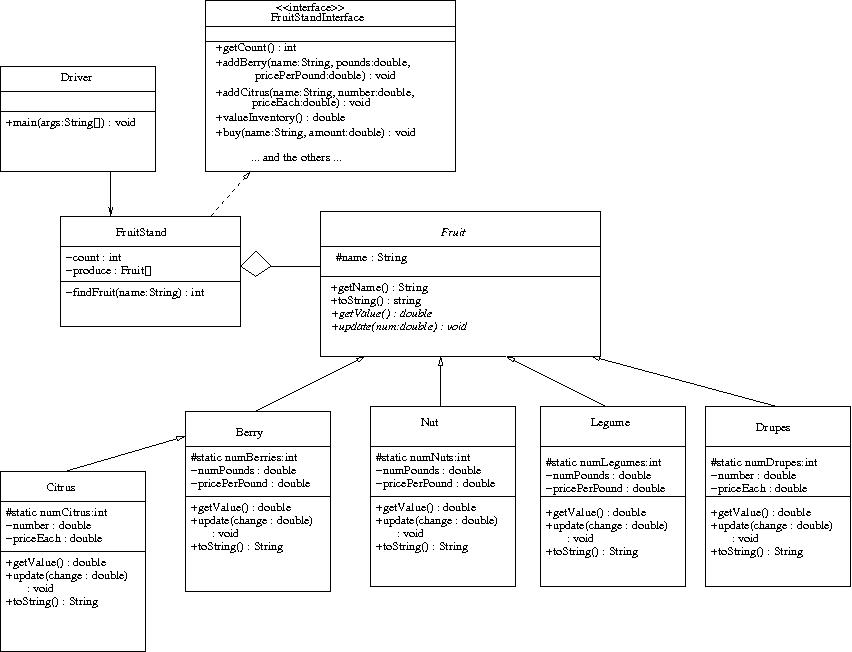
\includegraphics{UML.jpg}
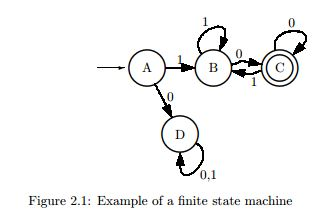
\includegraphics{29.jpg}
\end{enumerate}
\subsection*{Pushdown Stack}
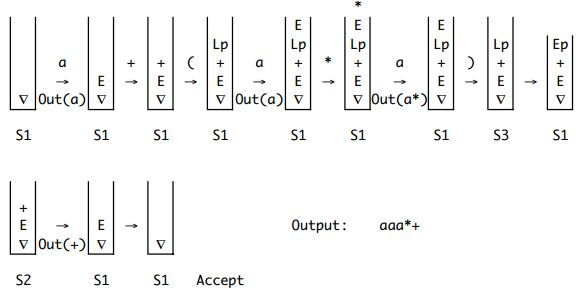
\includegraphics{80.jpg}
\subsection*{Linked List}
\subsection*{Hash Table}
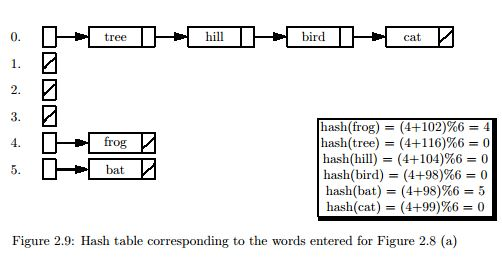
\includegraphics{48.jpg}
\subsection*{Trees}
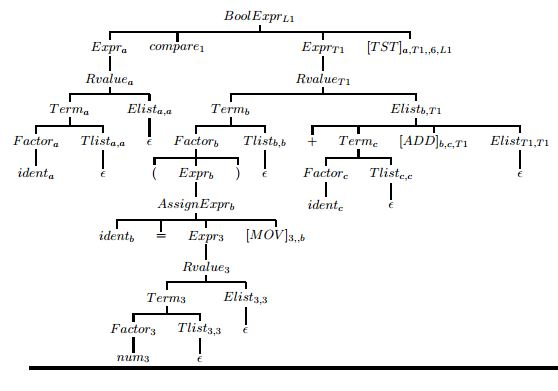
\includegraphics{148.jpg}
\subsection*{Syntax Diagram}
\includegraphics{if_statement.gif}

\end{flushleft}
%_______________________________________________

%%matts stuff
\begin{flushleft}
%%%%%%%%%%OBJECT DIAGRAM
\begin {figure}
\Draw


\MinNodeSize (20,10)
\ArrowHeads(1)
\ArrowSpec(F,10,4,5)
%% \DecVar \MaxX

%% Display the primitive values in an object
%% Called once for each primitive field
\Define \Var(3)
{	
%% parms:
%%    #1: 0 if this var has no primitive value
%%    #2: name of the var
%%    #3: value in a box
	
   \IF \GtInt (#1,0)  \THEN
	\MarkLoc(left)
 	\Move(0,-27)
	\EntryExit(-1,0,-1,0)
	\Node (tag) (--#2--)
	%% Note the longest field value, to draw the box
	{ 
	\MoveToExit(1,0)
	  \ORectNode (tag) (--#3--)
	\MoveToExit(1,0)  \MarkLoc(right)
	\Move(50,0)  \MarkLoc(rightPlus) 
	\MoveToLL(right,rightPlus)(topL,maxL)
	\MarkGLoc(bottomL)  
	\LSeg\Q(maxL,maxRight)
	\LSeg\R(bottomL,right)
	\IF \GtDec (\R,\Q) \THEN
	    \MoveToLoc(right)
	    \MarkGLoc(maxRight)
	    \FI
	}
	\EntryExit(0,0,0,0)
\MarkGLoc(bottom)
   \FI
}


%% Display the object references in an object
%% Called once for each primitive field
%% Object is a recursive data structure
\Define \Obj(8)
{	
%% parms:
%%    #1: 0 do not display
%%        1 display ordinary ref
%%	  2 display ref in a set
%%        3 display a key in a map
%%        4 display a ref to a set
%%        5 display a ref to a map
%%  	  6 display object only, calling OD directly, no arrow
%%    #2: name of the field
%%    #3: class of the field  (for object types)
%%    #4: table of primitive fields in the referred object
%% 	   or size for a map
%%    #5: table of object fields in the referred object
%%         or table of primitive keys for maps
%%    #6: table of object keys in the referred object
%%    #7: table of primitive values in the referred object
%%    #8: table of object values in the referred object

  % Base case for recursion:  #1 = 0

\IF \GtInt (#1, 0) \THEN		% Recursive case
					% for ordinary field or value in map

   \Move(0,-25)
   \MarkLoc(tmp)
   \EntryExit(-1,0,1.1,0)
   \Node (tag) (--#2--)
   \ORectNode(ref) (-- --)
   \EntryExit(0,0,0,0)
   \IF \EqInt(#1,1) \THEN		% ordinary ref
      \Move(100,\Val\I)
      \OD(#3, #4, #5, 1)  
   \FI
   \IF \EqInt(#1,2) \THEN		% ref in a set
 	\ODset(#3,#4,#5)
   \FI
   \IF \EqInt(#1,3) \THEN		% key in a map
	    \Move(-160,\Val\I)
	    \Move(0,-10)    
	    \OD(#3, #4, #5,3)  
   \FI
   \IF \EqInt(#1,4) \THEN		% ref to a set
	       \OD(#3,#4,#5,4)
   \FI
   \IF \EqInt(#1,5) \THEN		% ref to a map
	          \ODmap(#3,#4,#5,#6,#7,#8,#1)
   \FI
   \MoveToLoc(tmp)
   \I-100;
   \MarkGLoc(bottom)
\FI
   }
 
%% Draw the object in a rectangular box
%% Show primitive values
%% Show references as arrows to objects
\Define \OD(4)
{  
%% parms:
%%    #1:  class of the object 
%%    #2:  table of primitive fields 
%%    #3:  table of object fields 
%%    #4:  See parm #1 for Obj above

   \SaveAll
%%%%  J is depth of recursion
\J+1;
\IF \GtInt (\J,2) \THEN
      \Move(-400,-200)
      \J=0;
    
\FI
\Move (-20,60)   %%% ???  
\Node(obj)(--\underline{#1}--)
%% topLeft and bottomRight are used to draw the rectangle
\MoveToExit(1.02,0)    \MarkGLoc(maxRight)   %% maxRight stores largest primitive
\MoveToExit(-1.2,1.2)  \MarkLoc(topLeft)
\Move (50,-70)
 
\MinNodeSize(30,15)
\PenSize(0.25pt)	%% Lightweight arrow, might cross over other objects

%% Draw the arrow for a reference
\IF \EqInt (#4,3) \THEN 	%% key in a map
     { \CurvedEdgeAt (ref,-0.8,0, obj,1,0.5)(180,0.6,90, 0.6) }
	\ELSE
	\IF \EqInt (#4,6) \THEN		%% calling OD directly 
		{ } 			%% no arrow
        \ELSE
     	{ \CurvedEdgeAt (ref,0.8,0, obj,-1,0.8)(0,0.6,180, 0.6) }
   	\FI
   \FI

\Move(-45,70)
\PenSize(0.75pt)

{\MarkGLoc (maxL) \Move (0,100) \MarkGLoc(topL) }

\Indirect <#2>(0,9) { \Var }		%% Draw primitive fields
\MarkLoc(bottomTemp)
\MoveToLoc(maxRight) \MarkLoc(maxRightLocal)
\MoveToLoc(bottomTemp)

\Indirect<#3>(0,8) { \Obj   }		%% Draw object fields

%% Set maxRightLocal in case there were no primitive fields
\Move(100,0) \MarkLoc(maxRightTemp)
\MoveToRightmost(maxRightLocal,maxRightTemp)
\MarkLoc(maxRightLocal)
{
%% Find bottom right corner of rectangle
\MoveToLoc(bottom)
\Move(100,0) \MarkLoc(bottomR)
\MoveToLoc(maxRightLocal) \Move(0,-100) \MarkLoc(rightB)
\MoveToLL(bottom,bottomR)(maxRightLocal,rightB)
\Move(10,-20) 
\MarkLoc(bottomRight)
\CSeg \DrawRect(bottomRight,topLeft)
}
   
   \RecallAll
\J-1;
}

%% Draw a ref to a Set
\Define \ObjSet(6)
{	
%% parms:
%%    #1: 0 iff this field has no Object ref
%%    #2: name of the field
%%    #3: class of the field  (for object types)
%%    #4: table of primitive fields in the referred object - wrappers or Strings
%%    #5: table of object fields in the referred object
%%    #6: size of the set 

  % Base case:  #1 = 0

\IF \GtInt (#1, 0) \THEN		% Recursive case
	\MarkLoc(tmp)
   	\Node (tag) (--#2--)
	\Move (50,0)
	\ORectNode(ref) (-- --)
	\Move(50,\Val\I)
	\Move (35,20)
	\ODset(#3, #4, #5,#6)  
	\MoveToLoc(tmp)
	\I-135;
   \FI
}

%% Draw a set with the refs at 'random' places in the box
\Define \ODset(4)    
{  
%% parms:
%%    #1:  class of the object
%%    #2:  table of primitive fields 
%%    #3:  table of object fields 
%%    #4:  size of the set        
   \SaveAll
  
\MinNodeSize (90,110)
\RectNode(obj)(-- #1~~~~~~~~~~~~~~~~~~~~~~~--)
\MinNodeSize (20,10)

{ \PenSize(0.25pt)	%% Lightweight arrow, might cross over other objects
  %% Draw arrow to this Set object
  \CurvedEdgeAt (ref,0.8,0, obj,-1,0.8)(10,0.6,180, 0.6) }
  \PenSize(0.75pt)
   \IntVar \X      
   \IntVar \Y

   \Move(-50,70)
   { \Line(110,0) }
   \Move (15,-15)
   \Node(tag)(--size--)
   \MoveToExit(1,0)
   \Move(25,0)
   \ORectNode(tag)(--#4--)
   \Move(-90,0)
   \MarkLoc(start)

%% Place the fields at seemingly random locations
   \Indirect <#2>(0,9) { 		%% Draw the primitive fields
 	\X+34;
 	\K=\X;
	\K/90;
	\K*90;
 	\X-\K;		%% x + 34 mod 90
	\Y+73;
	\K=\Y;
	\K/110;
	\K*110;
	\Y-\K;		%% y + 73 mod 110
	\Y+20;		%% Allow for size at top
 		\MoveToLoc(start)
		\Move (\Val\X,-\Val\Y)
 		\Var
}

%% Place the fields at seemingly random locations
   \Indirect<#3>(0,9) { 		%% Draw the object fields
 	\X+34;
 	\K=\X;
 	\K/90;
 	\K*90;
 	\X-\K;		%% x + 72 mod 90
	\Y+73;
	\K=\Y;
	\K/110;
	\K*110;
	\Y-\K;		%% y + 73 mod 110
	\Y+20;		%% Allow for size at top
 	\MoveToLoc(start)
	\Move (\Val\X,-\Val\Y)
		 \Obj   
	}
   \RecallAll
}

%% Draw a map object in a rectangle
%% Value refs point to the right
%% Key refs point to the left
%% Note largest value field to draw the rectangle
\Define \ODmap(7)
{  
%% parms:
%%    #1:  class of the object 
%%    #2:  size
%%    #3:  table of primitive keys 
%%    #4:  table of object keys 
%%    #5:  table of primitive values 
%%    #6:  table of object values 
%%    #7:  see parm #1 for Obj above
   \SaveAll
  
\Move(-20,-60) 
\Node(obj)(--\underline{#1}--)
\MoveToExit(1.02,0) 	\MarkLoc (maxRightLocal)
			\MarkLoc (maxRight)
\MoveToExit(-1.2,1.2)\MarkLoc (topLeft)

\MinNodeSize(30,15)
\PenSize(0.25pt)		%% Use Lightweight pen, may cross other objects

\IF \EqInt(#7,3) \THEN
     \CurvedEdgeAt (ref,-0.8,0, obj,1,0.5)(180,0.6,90, 0.6) 
     \ELSE
	\IF \EqInt(#7,6) \THEN		%% calling ODmap directly
	    {  }
	\ELSE
	  \CurvedEdgeAt (ref,0.8,0, obj,-1,0.8)(10,0.6,180, 0.6) 
        \FI
\FI
	
\PenSize(0.75pt)
\Move(20,-35)
   
   %% Show size and headings for keys and values
   { \Node(tag)(--size--) \Move(40,0) \ORectNode(tag)(--#2--) }
   \Move (10,-20)
   { \Node(tag)(--\underline{keys}--) 
     \Move(75,0) \Node(tag)(--\underline {values}--) 
   }
   \Move (-50,0)
   \MarkLoc(keys)

   {\MarkGLoc (maxL) \Move (0,100) \MarkGLoc(topL) }   %% ??

  %% keys 
   \Indirect <#3>(0,9) { \Var  }	%% Draw the primitive keys

   \Indirect<#4>(0,8) { \Obj   }	%% Draw the object keys
   \MarkGLoc(bottom)
\MoveToLoc(keys)
\Move(83, -1)
{
  %% values 
   \Indirect <#5>(0,9) { \Var  }	%% Draw the primitive values
   \MarkLoc(bottomTemp)
   \MoveToLoc(bottomTemp)

   \Indirect<#6>(0,8) { \Obj   }	%% Draw the object values

%% Keys may not be primitive, affects size of box
\Move(100,0)	\MarkLoc(maxRightTemp)
\MoveToRightmost(maxRightLocal,maxRightTemp)
\MarkLoc(maxRightLocal)
}
{
%% Find bottom right corner of rectangle
\MoveToLoc(bottom)
\Move(100,0)	\MarkLoc(bottomR)
\MoveToLoc(maxRightLocal)	\Move(0,-100)	\MarkLoc(rightB)
\MoveToLL(bottom,bottomR)(maxRightLocal,rightB)
\Move(10,-20)
\MarkLoc(bottomRight)
\CSeg \DrawRect(bottomRight,topLeft)
}
   \RecallAll
}

%% Move the pen to the loc which is furthest right
\Define \MoveToRightmost(2)
{
%% #1:  A loc
%% #2:  A loc
\MoveTo(-200,100)	\MarkLoc(upLeft)
\MoveTo(-200,-100)	\MarkLoc(downLeft)
\MoveToLoc(#1)		\Move(100,0)	\MarkLoc(right)
\MoveToLL(upLeft,downLeft)(#1,right)	\MarkLoc(leftA)
\MoveToLoc(#2)		\Move(100,0)	\MarkLoc(right)
\MoveToLL(upLeft,downLeft)(#2,right)	\MarkLoc(leftB)

	\LSeg\Q(leftA,#1)
	\LSeg\R(leftB,#2)
	\MoveToLoc(#1)
	\IF \GtDec (\R,\Q) \THEN
	    \MoveToLoc(#2)
	    \FI
}

\Indirect \Table <studentPrims>
{  1, info, "1" 		&
   1, info2,  "2"		&
   1, info3,  "3"		
}
\Indirect \Table <studentObjs>
 {  0, home,Address,addrAPrims,addrAObjs, , , }
  \Scale (0.8,0.8)
\OD (OBJECT NAME, studentPrims, studentObjs, 6)
    \EndDraw
\caption {CAPTION HERE}
\label {fig:simpleStudent}
\end {figure}

\subsection*{Arrays}

%%ARRAY EXAMPLE 
%%User Input Below
\newcommand{\ArrayName}
{ARRAY NAME HERE}
\newcommand{\Caption}
{CAPTION HERE}
\newcommand{\ArrayLengthMinusOne}
{6}
\newcommand{\0}
{0}
\newcommand{\1}
{0}
\newcommand{\2}
{95}
\newcommand{\3}
{0}
\newcommand{\4}
{0}
\newcommand{\5}
{0}
\newcommand{\6}
{0}
\newcommand{\7}
{0}
\newcommand{\8}
{0}
\newcommand{\9}
{0}
\newcommand{\ten}
{0}
\newcommand{\eleven}
{0}
%%User Input Above
\begin {figure}

\Draw



\MinNodeSize (20,10)
\ArrowHeads(1)
\ArrowSpec(F,10,4,5)
%% \DecVar \MaxX

%% Display the primitive values in an object
%% Called once for each primitive field
\Define \Var(3)
{	
%% parms:
%%    #1: 0 if this var has no primitive value
%%    #2: name of the var
%%    #3: value in a box
	
   \IF \GtInt (#1,0)  \THEN
	\MarkLoc(left)
 	\Move(0,-27)
	\EntryExit(-1,0,-1,0)
	\Node (tag) (--#2--)
	%% Note the longest field value, to draw the box
	{ 
	\MoveToExit(1,0)
	  \ORectNode (tag) (--#3--)
	\MoveToExit(1,0)  \MarkLoc(right)
	\Move(50,0)  \MarkLoc(rightPlus) 
	\MoveToLL(right,rightPlus)(topL,maxL)
	\MarkGLoc(bottomL)  
	\LSeg\Q(maxL,maxRight)
	\LSeg\R(bottomL,right)
	\IF \GtDec (\R,\Q) \THEN
	    \MoveToLoc(right)
	    \MarkGLoc(maxRight)
	    \FI
	}
	\EntryExit(0,0,0,0)
\MarkGLoc(bottom)
   \FI
}


%% Display the object references in an object
%% Called once for each primitive field
%% Object is a recursive data structure
\Define \Obj(8)
{	
%% parms:
%%    #1: 0 do not display
%%        1 display ordinary ref
%%	  2 display ref in a set
%%        3 display a key in a map
%%        4 display a ref to a set
%%        5 display a ref to a map
%%  	  6 display object only, calling OD directly, no arrow
%%    #2: name of the field
%%    #3: class of the field  (for object types)
%%    #4: table of primitive fields in the referred object
%% 	   or size for a map
%%    #5: table of object fields in the referred object
%%         or table of primitive keys for maps
%%    #6: table of object keys in the referred object
%%    #7: table of primitive values in the referred object
%%    #8: table of object values in the referred object

  % Base case for recursion:  #1 = 0

\IF \GtInt (#1, 0) \THEN		% Recursive case
					% for ordinary field or value in map

   \Move(0,-25)
   \MarkLoc(tmp)
   \EntryExit(-1,0,1.1,0)
   \Node (tag) (--#2--)
   \ORectNode(ref) (-- --)
   \EntryExit(0,0,0,0)
   \IF \EqInt(#1,1) \THEN		% ordinary ref
      \Move(100,\Val\I)
      \OD(#3, #4, #5, 1)  
   \FI
   \IF \EqInt(#1,2) \THEN		% ref in a set
 	\ODset(#3,#4,#5)
   \FI
   \IF \EqInt(#1,3) \THEN		% key in a map
	    \Move(-160,\Val\I)
	    \Move(0,-10)    
	    \OD(#3, #4, #5,3)  
   \FI
   \IF \EqInt(#1,4) \THEN		% ref to a set
	       \OD(#3,#4,#5,4)
   \FI
   \IF \EqInt(#1,5) \THEN		% ref to a map
	          \ODmap(#3,#4,#5,#6,#7,#8,#1)
   \FI
   \MoveToLoc(tmp)
   \I-100;
   \MarkGLoc(bottom)
\FI
   }
 
%% Draw the object in a rectangular box
%% Show primitive values
%% Show references as arrows to objects
\Define \OD(4)
{  
%% parms:
%%    #1:  class of the object 
%%    #2:  table of primitive fields 
%%    #3:  table of object fields 
%%    #4:  See parm #1 for Obj above

   \SaveAll
%%%%  J is depth of recursion
\J+1;
\IF \GtInt (\J,2) \THEN
      \Move(-400,-200)
      \J=0;
    
\FI
\Move (-20,60)   %%% ???  
\Node(obj)(--\underline{#1}--)
%% topLeft and bottomRight are used to draw the rectangle
\MoveToExit(1.02,0)    \MarkGLoc(maxRight)   %% maxRight stores largest primitive
\MoveToExit(-1.2,1.2)  \MarkLoc(topLeft)
\Move (50,-70)
 
\MinNodeSize(30,15)
\PenSize(0.25pt)	%% Lightweight arrow, might cross over other objects

%% Draw the arrow for a reference
\IF \EqInt (#4,3) \THEN 	%% key in a map
     { \CurvedEdgeAt (ref,-0.8,0, obj,1,0.5)(180,0.6,90, 0.6) }
	\ELSE
	\IF \EqInt (#4,6) \THEN		%% calling OD directly 
		{ } 			%% no arrow
        \ELSE
     	{ \CurvedEdgeAt (ref,0.8,0, obj,-1,0.8)(0,0.6,180, 0.6) }
   	\FI
   \FI

\Move(-45,70)
\PenSize(0.75pt)

{\MarkGLoc (maxL) \Move (0,100) \MarkGLoc(topL) }

\Indirect <#2>(0,9) { \Var }		%% Draw primitive fields
\MarkLoc(bottomTemp)
\MoveToLoc(maxRight) \MarkLoc(maxRightLocal)
\MoveToLoc(bottomTemp)

\Indirect<#3>(0,8) { \Obj   }		%% Draw object fields

%% Set maxRightLocal in case there were no primitive fields
\Move(100,0) \MarkLoc(maxRightTemp)
\MoveToRightmost(maxRightLocal,maxRightTemp)
\MarkLoc(maxRightLocal)
{
%% Find bottom right corner of rectangle
\MoveToLoc(bottom)
\Move(100,0) \MarkLoc(bottomR)
\MoveToLoc(maxRightLocal) \Move(0,-100) \MarkLoc(rightB)
\MoveToLL(bottom,bottomR)(maxRightLocal,rightB)
\Move(10,-20) 
\MarkLoc(bottomRight)
\CSeg \DrawRect(bottomRight,topLeft)
}
   
   \RecallAll
\J-1;
}

%% Draw a ref to a Set
\Define \ObjSet(6)
{	
%% parms:
%%    #1: 0 iff this field has no Object ref
%%    #2: name of the field
%%    #3: class of the field  (for object types)
%%    #4: table of primitive fields in the referred object - wrappers or Strings
%%    #5: table of object fields in the referred object
%%    #6: size of the set 

  % Base case:  #1 = 0

\IF \GtInt (#1, 0) \THEN		% Recursive case
	\MarkLoc(tmp)
   	\Node (tag) (--#2--)
	\Move (50,0)
	\ORectNode(ref) (-- --)
	\Move(50,\Val\I)
	\Move (35,20)
	\ODset(#3, #4, #5,#6)  
	\MoveToLoc(tmp)
	\I-135;
   \FI
}

%% Draw a set with the refs at 'random' places in the box
\Define \ODset(4)    
{  
%% parms:
%%    #1:  class of the object
%%    #2:  table of primitive fields 
%%    #3:  table of object fields 
%%    #4:  size of the set        
   \SaveAll
  
\MinNodeSize (90,110)
\RectNode(obj)(-- #1~~~~~~~~~~~~~~~~~~~~~~~--)
\MinNodeSize (20,10)

{ \PenSize(0.25pt)	%% Lightweight arrow, might cross over other objects
  %% Draw arrow to this Set object
  \CurvedEdgeAt (ref,0.8,0, obj,-1,0.8)(10,0.6,180, 0.6) }
  \PenSize(0.75pt)
   \IntVar \X      
   \IntVar \Y

   \Move(-50,70)
   { \Line(110,0) }
   \Move (15,-15)
   \Node(tag)(--size--)
   \MoveToExit(1,0)
   \Move(25,0)
   \ORectNode(tag)(--#4--)
   \Move(-90,0)
   \MarkLoc(start)

%% Place the fields at seemingly random locations
   \Indirect <#2>(0,9) { 		%% Draw the primitive fields
 	\X+34;
 	\K=\X;
	\K/90;
	\K*90;
 	\X-\K;		%% x + 34 mod 90
	\Y+73;
	\K=\Y;
	\K/110;
	\K*110;
	\Y-\K;		%% y + 73 mod 110
	\Y+20;		%% Allow for size at top
 		\MoveToLoc(start)
		\Move (\Val\X,-\Val\Y)
 		\Var
}

%% Place the fields at seemingly random locations
   \Indirect<#3>(0,9) { 		%% Draw the object fields
 	\X+34;
 	\K=\X;
 	\K/90;
 	\K*90;
 	\X-\K;		%% x + 72 mod 90
	\Y+73;
	\K=\Y;
	\K/110;
	\K*110;
	\Y-\K;		%% y + 73 mod 110
	\Y+20;		%% Allow for size at top
 	\MoveToLoc(start)
	\Move (\Val\X,-\Val\Y)
		 \Obj   
	}
   \RecallAll
}

%% Draw a map object in a rectangle
%% Value refs point to the right
%% Key refs point to the left
%% Note largest value field to draw the rectangle
\Define \ODmap(7)
{  
%% parms:
%%    #1:  class of the object 
%%    #2:  size
%%    #3:  table of primitive keys 
%%    #4:  table of object keys 
%%    #5:  table of primitive values 
%%    #6:  table of object values 
%%    #7:  see parm #1 for Obj above
   \SaveAll
  
\Move(-20,-60) 
\Node(obj)(--\underline{#1}--)
\MoveToExit(1.02,0) 	\MarkLoc (maxRightLocal)
			\MarkLoc (maxRight)
\MoveToExit(-1.2,1.2)\MarkLoc (topLeft)

\MinNodeSize(30,15)
\PenSize(0.25pt)		%% Use Lightweight pen, may cross other objects

\IF \EqInt(#7,3) \THEN
     \CurvedEdgeAt (ref,-0.8,0, obj,1,0.5)(180,0.6,90, 0.6) 
     \ELSE
	\IF \EqInt(#7,6) \THEN		%% calling ODmap directly
	    {  }
	\ELSE
	  \CurvedEdgeAt (ref,0.8,0, obj,-1,0.8)(10,0.6,180, 0.6) 
        \FI
\FI
	
\PenSize(0.75pt)
\Move(20,-35)
   
   %% Show size and headings for keys and values
   { \Node(tag)(--size--) \Move(40,0) \ORectNode(tag)(--#2--) }
   \Move (10,-20)
   { \Node(tag)(--\underline{keys}--) 
     \Move(75,0) \Node(tag)(--\underline {values}--) 
   }
   \Move (-50,0)
   \MarkLoc(keys)

   {\MarkGLoc (maxL) \Move (0,100) \MarkGLoc(topL) }   %% ??

  %% keys 
   \Indirect <#3>(0,9) { \Var  }	%% Draw the primitive keys

   \Indirect<#4>(0,8) { \Obj   }	%% Draw the object keys
   \MarkGLoc(bottom)
\MoveToLoc(keys)
\Move(83, -1)
{
  %% values 
   \Indirect <#5>(0,9) { \Var  }	%% Draw the primitive values
   \MarkLoc(bottomTemp)
   \MoveToLoc(bottomTemp)

   \Indirect<#6>(0,8) { \Obj   }	%% Draw the object values

%% Keys may not be primitive, affects size of box
\Move(100,0)	\MarkLoc(maxRightTemp)
\MoveToRightmost(maxRightLocal,maxRightTemp)
\MarkLoc(maxRightLocal)
}
{
%% Find bottom right corner of rectangle
\MoveToLoc(bottom)
\Move(100,0)	\MarkLoc(bottomR)
\MoveToLoc(maxRightLocal)	\Move(0,-100)	\MarkLoc(rightB)
\MoveToLL(bottom,bottomR)(maxRightLocal,rightB)
\Move(10,-20)
\MarkLoc(bottomRight)
\CSeg \DrawRect(bottomRight,topLeft)
}
   \RecallAll
}

%% Move the pen to the loc which is furthest right
\Define \MoveToRightmost(2)
{
%% #1:  A loc
%% #2:  A loc
\MoveTo(-200,100)	\MarkLoc(upLeft)
\MoveTo(-200,-100)	\MarkLoc(downLeft)
\MoveToLoc(#1)		\Move(100,0)	\MarkLoc(right)
\MoveToLL(upLeft,downLeft)(#1,right)	\MarkLoc(leftA)
\MoveToLoc(#2)		\Move(100,0)	\MarkLoc(right)
\MoveToLL(upLeft,downLeft)(#2,right)	\MarkLoc(leftB)

	\LSeg\Q(leftA,#1)
	\LSeg\R(leftB,#2)
	\MoveToLoc(#1)
	\IF \GtDec (\R,\Q) \THEN
	    \MoveToLoc(#2)
	    \FI
}

%%Array Name Draw
\Move(-50,0)
\Node(tag)(--\ArrayName--)
\MoveToExit(1,0)
\Move(20,0)
\ORectNode(gr)(----)
\Move (25,-25)

%%Array Draw
\MinNodeSize(20,20)
\Node(start)(----)
%%\newcounter{Counter}

\Do(0,\ArrayLengthMinusOne)
{  
	\IF 
    	\EqInt(0,0) 				
        	\THEN
 				\RectNode(rec)(--0--)
                %%\stepcounter{Counter}
   \ELSE
   		\RectNode(rec)(--1--)
   		
 		   \FI
   { 	\MoveToExit(0,-1.8)
 	\Node(tag)(--\DoReg--)
   }
   \MoveToExit(2,0)
}
%%Arrow
\ArrowHeads(1)
\CurvedEdgeAt(gr,0,-0.5,start,-1,0) (-90,0.2,180,0.2)
\EndDraw
\caption {\Caption}
\label {fig:array}
\end {figure}

With Arrays the user will be able to input the information for the array name, caption name, length of the array and the actual values of the array.  

\subsection*{Expressions}

%%Expression Example
\begin {figure}
\Draw
\input boxIt
\input boxIt
\MarkLoc(a)
\Move(50,0)
\MarkLoc(b)
\Move(75,0)
\MarkLoc(c)
\boxItDefault(4,2,a)
\boxItDefault(3,2,b)
\boxItDefault(4,4,c)
\MoveToLoc(a)
\Move(25,0)
\MarkLoc(d)
\boxIt(~$  +  $~,2,d,105, 25)
\boxIt(\hspace{135pt}\hfill*\hspace{10pt},4,d, 250, 35)
\EndDraw
\caption {CAPTION HERE }
\label {fig:exprsBoxedAmb1}
\end {figure}

With Expressions the user will be able to edit the caption name, ??????

\subsection*{Classes}

%%Classes Example
\begin {figure}
\Draw


\MinNodeSize (20,10)
\ArrowHeads(1)
\ArrowSpec(F,10,4,5)
%% \DecVar \MaxX

%% Display the primitive values in an object
%% Called once for each primitive field
\Define \Var(3)
{	
%% parms:
%%    #1: 0 if this var has no primitive value
%%    #2: name of the var
%%    #3: value in a box
	
   \IF \GtInt (#1,0)  \THEN
	\MarkLoc(left)
 	\Move(0,-27)
	\EntryExit(-1,0,-1,0)
	\Node (tag) (--#2--)
	%% Note the longest field value, to draw the box
	{ 
	\MoveToExit(1,0)
	  \ORectNode (tag) (--#3--)
	\MoveToExit(1,0)  \MarkLoc(right)
	\Move(50,0)  \MarkLoc(rightPlus) 
	\MoveToLL(right,rightPlus)(topL,maxL)
	\MarkGLoc(bottomL)  
	\LSeg\Q(maxL,maxRight)
	\LSeg\R(bottomL,right)
	\IF \GtDec (\R,\Q) \THEN
	    \MoveToLoc(right)
	    \MarkGLoc(maxRight)
	    \FI
	}
	\EntryExit(0,0,0,0)
\MarkGLoc(bottom)
   \FI
}


%% Display the object references in an object
%% Called once for each primitive field
%% Object is a recursive data structure
\Define \Obj(8)
{	
%% parms:
%%    #1: 0 do not display
%%        1 display ordinary ref
%%	  2 display ref in a set
%%        3 display a key in a map
%%        4 display a ref to a set
%%        5 display a ref to a map
%%  	  6 display object only, calling OD directly, no arrow
%%    #2: name of the field
%%    #3: class of the field  (for object types)
%%    #4: table of primitive fields in the referred object
%% 	   or size for a map
%%    #5: table of object fields in the referred object
%%         or table of primitive keys for maps
%%    #6: table of object keys in the referred object
%%    #7: table of primitive values in the referred object
%%    #8: table of object values in the referred object

  % Base case for recursion:  #1 = 0

\IF \GtInt (#1, 0) \THEN		% Recursive case
					% for ordinary field or value in map

   \Move(0,-25)
   \MarkLoc(tmp)
   \EntryExit(-1,0,1.1,0)
   \Node (tag) (--#2--)
   \ORectNode(ref) (-- --)
   \EntryExit(0,0,0,0)
   \IF \EqInt(#1,1) \THEN		% ordinary ref
      \Move(100,\Val\I)
      \OD(#3, #4, #5, 1)  
   \FI
   \IF \EqInt(#1,2) \THEN		% ref in a set
 	\ODset(#3,#4,#5)
   \FI
   \IF \EqInt(#1,3) \THEN		% key in a map
	    \Move(-160,\Val\I)
	    \Move(0,-10)    
	    \OD(#3, #4, #5,3)  
   \FI
   \IF \EqInt(#1,4) \THEN		% ref to a set
	       \OD(#3,#4,#5,4)
   \FI
   \IF \EqInt(#1,5) \THEN		% ref to a map
	          \ODmap(#3,#4,#5,#6,#7,#8,#1)
   \FI
   \MoveToLoc(tmp)
   \I-100;
   \MarkGLoc(bottom)
\FI
   }
 
%% Draw the object in a rectangular box
%% Show primitive values
%% Show references as arrows to objects
\Define \OD(4)
{  
%% parms:
%%    #1:  class of the object 
%%    #2:  table of primitive fields 
%%    #3:  table of object fields 
%%    #4:  See parm #1 for Obj above

   \SaveAll
%%%%  J is depth of recursion
\J+1;
\IF \GtInt (\J,2) \THEN
      \Move(-400,-200)
      \J=0;
    
\FI
\Move (-20,60)   %%% ???  
\Node(obj)(--\underline{#1}--)
%% topLeft and bottomRight are used to draw the rectangle
\MoveToExit(1.02,0)    \MarkGLoc(maxRight)   %% maxRight stores largest primitive
\MoveToExit(-1.2,1.2)  \MarkLoc(topLeft)
\Move (50,-70)
 
\MinNodeSize(30,15)
\PenSize(0.25pt)	%% Lightweight arrow, might cross over other objects

%% Draw the arrow for a reference
\IF \EqInt (#4,3) \THEN 	%% key in a map
     { \CurvedEdgeAt (ref,-0.8,0, obj,1,0.5)(180,0.6,90, 0.6) }
	\ELSE
	\IF \EqInt (#4,6) \THEN		%% calling OD directly 
		{ } 			%% no arrow
        \ELSE
     	{ \CurvedEdgeAt (ref,0.8,0, obj,-1,0.8)(0,0.6,180, 0.6) }
   	\FI
   \FI

\Move(-45,70)
\PenSize(0.75pt)

{\MarkGLoc (maxL) \Move (0,100) \MarkGLoc(topL) }

\Indirect <#2>(0,9) { \Var }		%% Draw primitive fields
\MarkLoc(bottomTemp)
\MoveToLoc(maxRight) \MarkLoc(maxRightLocal)
\MoveToLoc(bottomTemp)

\Indirect<#3>(0,8) { \Obj   }		%% Draw object fields

%% Set maxRightLocal in case there were no primitive fields
\Move(100,0) \MarkLoc(maxRightTemp)
\MoveToRightmost(maxRightLocal,maxRightTemp)
\MarkLoc(maxRightLocal)
{
%% Find bottom right corner of rectangle
\MoveToLoc(bottom)
\Move(100,0) \MarkLoc(bottomR)
\MoveToLoc(maxRightLocal) \Move(0,-100) \MarkLoc(rightB)
\MoveToLL(bottom,bottomR)(maxRightLocal,rightB)
\Move(10,-20) 
\MarkLoc(bottomRight)
\CSeg \DrawRect(bottomRight,topLeft)
}
   
   \RecallAll
\J-1;
}

%% Draw a ref to a Set
\Define \ObjSet(6)
{	
%% parms:
%%    #1: 0 iff this field has no Object ref
%%    #2: name of the field
%%    #3: class of the field  (for object types)
%%    #4: table of primitive fields in the referred object - wrappers or Strings
%%    #5: table of object fields in the referred object
%%    #6: size of the set 

  % Base case:  #1 = 0

\IF \GtInt (#1, 0) \THEN		% Recursive case
	\MarkLoc(tmp)
   	\Node (tag) (--#2--)
	\Move (50,0)
	\ORectNode(ref) (-- --)
	\Move(50,\Val\I)
	\Move (35,20)
	\ODset(#3, #4, #5,#6)  
	\MoveToLoc(tmp)
	\I-135;
   \FI
}

%% Draw a set with the refs at 'random' places in the box
\Define \ODset(4)    
{  
%% parms:
%%    #1:  class of the object
%%    #2:  table of primitive fields 
%%    #3:  table of object fields 
%%    #4:  size of the set        
   \SaveAll
  
\MinNodeSize (90,110)
\RectNode(obj)(-- #1~~~~~~~~~~~~~~~~~~~~~~~--)
\MinNodeSize (20,10)

{ \PenSize(0.25pt)	%% Lightweight arrow, might cross over other objects
  %% Draw arrow to this Set object
  \CurvedEdgeAt (ref,0.8,0, obj,-1,0.8)(10,0.6,180, 0.6) }
  \PenSize(0.75pt)
   \IntVar \X      
   \IntVar \Y

   \Move(-50,70)
   { \Line(110,0) }
   \Move (15,-15)
   \Node(tag)(--size--)
   \MoveToExit(1,0)
   \Move(25,0)
   \ORectNode(tag)(--#4--)
   \Move(-90,0)
   \MarkLoc(start)

%% Place the fields at seemingly random locations
   \Indirect <#2>(0,9) { 		%% Draw the primitive fields
 	\X+34;
 	\K=\X;
	\K/90;
	\K*90;
 	\X-\K;		%% x + 34 mod 90
	\Y+73;
	\K=\Y;
	\K/110;
	\K*110;
	\Y-\K;		%% y + 73 mod 110
	\Y+20;		%% Allow for size at top
 		\MoveToLoc(start)
		\Move (\Val\X,-\Val\Y)
 		\Var
}

%% Place the fields at seemingly random locations
   \Indirect<#3>(0,9) { 		%% Draw the object fields
 	\X+34;
 	\K=\X;
 	\K/90;
 	\K*90;
 	\X-\K;		%% x + 72 mod 90
	\Y+73;
	\K=\Y;
	\K/110;
	\K*110;
	\Y-\K;		%% y + 73 mod 110
	\Y+20;		%% Allow for size at top
 	\MoveToLoc(start)
	\Move (\Val\X,-\Val\Y)
		 \Obj   
	}
   \RecallAll
}

%% Draw a map object in a rectangle
%% Value refs point to the right
%% Key refs point to the left
%% Note largest value field to draw the rectangle
\Define \ODmap(7)
{  
%% parms:
%%    #1:  class of the object 
%%    #2:  size
%%    #3:  table of primitive keys 
%%    #4:  table of object keys 
%%    #5:  table of primitive values 
%%    #6:  table of object values 
%%    #7:  see parm #1 for Obj above
   \SaveAll
  
\Move(-20,-60) 
\Node(obj)(--\underline{#1}--)
\MoveToExit(1.02,0) 	\MarkLoc (maxRightLocal)
			\MarkLoc (maxRight)
\MoveToExit(-1.2,1.2)\MarkLoc (topLeft)

\MinNodeSize(30,15)
\PenSize(0.25pt)		%% Use Lightweight pen, may cross other objects

\IF \EqInt(#7,3) \THEN
     \CurvedEdgeAt (ref,-0.8,0, obj,1,0.5)(180,0.6,90, 0.6) 
     \ELSE
	\IF \EqInt(#7,6) \THEN		%% calling ODmap directly
	    {  }
	\ELSE
	  \CurvedEdgeAt (ref,0.8,0, obj,-1,0.8)(10,0.6,180, 0.6) 
        \FI
\FI
	
\PenSize(0.75pt)
\Move(20,-35)
   
   %% Show size and headings for keys and values
   { \Node(tag)(--size--) \Move(40,0) \ORectNode(tag)(--#2--) }
   \Move (10,-20)
   { \Node(tag)(--\underline{keys}--) 
     \Move(75,0) \Node(tag)(--\underline {values}--) 
   }
   \Move (-50,0)
   \MarkLoc(keys)

   {\MarkGLoc (maxL) \Move (0,100) \MarkGLoc(topL) }   %% ??

  %% keys 
   \Indirect <#3>(0,9) { \Var  }	%% Draw the primitive keys

   \Indirect<#4>(0,8) { \Obj   }	%% Draw the object keys
   \MarkGLoc(bottom)
\MoveToLoc(keys)
\Move(83, -1)
{
  %% values 
   \Indirect <#5>(0,9) { \Var  }	%% Draw the primitive values
   \MarkLoc(bottomTemp)
   \MoveToLoc(bottomTemp)

   \Indirect<#6>(0,8) { \Obj   }	%% Draw the object values

%% Keys may not be primitive, affects size of box
\Move(100,0)	\MarkLoc(maxRightTemp)
\MoveToRightmost(maxRightLocal,maxRightTemp)
\MarkLoc(maxRightLocal)
}
{
%% Find bottom right corner of rectangle
\MoveToLoc(bottom)
\Move(100,0)	\MarkLoc(bottomR)
\MoveToLoc(maxRightLocal)	\Move(0,-100)	\MarkLoc(rightB)
\MoveToLL(bottom,bottomR)(maxRightLocal,rightB)
\Move(10,-20)
\MarkLoc(bottomRight)
\CSeg \DrawRect(bottomRight,topLeft)
}
   \RecallAll
}

%% Move the pen to the loc which is furthest right
\Define \MoveToRightmost(2)
{
%% #1:  A loc
%% #2:  A loc
\MoveTo(-200,100)	\MarkLoc(upLeft)
\MoveTo(-200,-100)	\MarkLoc(downLeft)
\MoveToLoc(#1)		\Move(100,0)	\MarkLoc(right)
\MoveToLL(upLeft,downLeft)(#1,right)	\MarkLoc(leftA)
\MoveToLoc(#2)		\Move(100,0)	\MarkLoc(right)
\MoveToLL(upLeft,downLeft)(#2,right)	\MarkLoc(leftB)

	\LSeg\Q(leftA,#1)
	\LSeg\R(leftB,#2)
	\MoveToLoc(#1)
	\IF \GtDec (\R,\Q) \THEN
	    \MoveToLoc(#2)
	    \FI
}

\MinNodeSize(40,40)
\RectNode (student)(--\underline {TOP}~~~~--)
\MoveToExit(-2,-3)
\RectNode (underGrad)(--\underline {TOPchild}~~~~--)
\MoveToExit(3,0)
\RectNode (gradStudent)(--\underline {TOPchild}~~~~--)
\ArrowSpec (H)
\Edge(underGrad,student)
\Edge(gradStudent,student)
\EndDraw
\caption {CAPTION HERE}
\label {fig:studentClasses}
\end {figure}

\section{User Input}
Users will be able to create diagrams by editing a section near the top of the latex code.  This section will be clearly defined, easily editedable and understandable.  Below is a work in progress of some latex code that the user will have to edit to create a diagram that fits their specs. The example below is specifically used when making array diagrams and is far from final.

\begin{quote}{\ttfamily \raggedright \noindent
User Input Below~\\
{\textbackslash}newcommand{\{}{\textbackslash}ArrayName{\}}~\\
{\{}ARRAY NAME HERE{\}}~\\
{\textbackslash}newcommand{\{}{\textbackslash}Caption{\}}~\\
{\{}CAPTION HERE{\}}~\\
{\textbackslash}newcommand{\{}{\textbackslash}ArrayLengthMinusOne{\}}~\\
{\{}ARRAY LENGTH HERE{\}}~\\
{\textbackslash}newcommand{\{}{\textbackslash}0{\}}~\\
{\{}PLACE 0 VALUE HERE{\}}~\\
{\textbackslash}newcommand{\{}{\textbackslash}1{\}}~\\
{\{}PLACE 1 VALUE HERE{\}}~\\
{\textbackslash}newcommand{\{}{\textbackslash}2{\}}~\\
{\{}PLACE 2 VALUE HERE{\}}~\\
{\textbackslash}newcommand{\{}{\textbackslash}3{\}}~\\
{\{}PLACE 3 VALUE HERE{\}}~\\
{\textbackslash}newcommand{\{}{\textbackslash}4{\}}~\\
{\{}PLACE 4 VALUE HERE{\}}~\\
User Input Above~\\
}\end{quote}

The user will find the location in the template that clearly states "User Input Below" and edit below that until they come to "User Input Above".  The user will edit only the statements that are in CAPS being careful not to edit anything besides that.  For example if the user wanted to create an array diagram that holds 4 values they would look for "ARRAY LENGTH HERE".  After finding this they would replace the text in CAPS with an integer.  The user would then compile the LATEX code to find a array diagram to the users specs.  Above the user input area there will be information regarding what inputs are acceptable for the template.

To declare a UML class/object diagram:
{\textbackslash}umlcobject{\{}
objectblock{object1,referenceType,referenceToObject/Objects},..,..,
{\}}~ \\

To declare a State,Stack, diagram:
{\textbackslash}statediagm{\{}table{\}}~ \\ 
Parameter table consist of states and input, and state reference for each input.

To declare a tree:
{\textbackslash}tree{\{}{\textbackslash}branch{\{}object,[]children{\}}, {\{}{\textbackslash}branch{object,[]children}{\}}~\\


\end{flushleft}

\pdfbookmark[1]{Change History}{change}
\newpage
\begin{multicols}{2} % Two-column layout throughout the main article text

\section*{Change History}
v0.1\\
\indent General: Initial version \dotfill 1
\end{multicols}

\end{document}
